documentclass[a4paper,11pt]{article}
usepackage[frenchb]{babel}
usepackage[T1]{fontenc}
usepackage[utf8]{inputenc}
usepackage{lmodern}
usepackage{microtype}

usepackage{array,multirow,makecell}
setcellgapes{1pt}
makegapedcells
usepackage{caption}
usepackage{adjustbox}

usepackage{amsmath,amssymb,bm,upgreek,stmaryrd,mathrsfs,systeme}

usepackage{graphicx}

usepackage{geometry}
geometry{hmargin=3cm,vmargin=2cm}

usepackage{hyperref}

\begin{document}

Constante de Steffan-Boltzmann:
\[\sigma = \frac{2\pi^{5}k^{4}}{15h^{3}c^{2}} \approx 5,670374419 \times 10^{-8} W \cdot m^{-2} \cdot K ^{-4}\[

Température du soleil $T_s$:
On remarque sur le graphe précedent qu'il existe un pic de $u(\lambda)$ et que selon la temperature $T$, le pic n'est pas à la meme longueur d'onde.

\begin{adjustbox}{center}
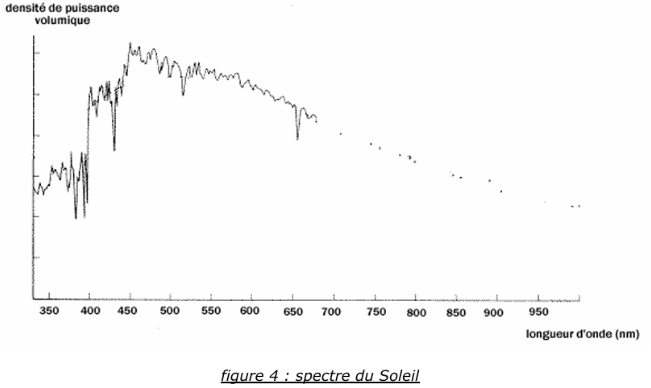
\includegraphics[scale=0.5]{densite_temperature}
\end{adjustbox}
\captionof{table}{Rotation de la Terre (vue de dessus) \\} 

La loi de déplacement de Wien donnne la longueur d'onde $\lambda_m$ pour laquelle on a le maximum de puissance en fonction de la température $T$.
\[\fbox{\lambda_m = \dfrac{hc}{4,96kT}} = \dfrac{2,898 \cdot 10^{-3}}{T}}}\]
avec $\lambda_{(Soleil)} = 500 nm$

En isolant $T$, on fait l'application numérique de la température du Soleil:
\[T_s= \dfrac{2.89 \times 10^{-3}}{500 \times 10^{-9}} = 5780 K \]



Distance Terre-Soleil $\d_{T-S}$:
L' unité astronomique (  AU ) est une unité de longueur définie pour être exactement égale à 149 597 870 700 m. Historiquement, l'unité astronomique était conçue comme la distance moyenne Terre-Soleil (la moyenne de l'aphélie et du périhélie de la Terre ), avant sa redéfinition moderne en 2012. 
On a donc d_{T-S} = 149 597 870 700 m.
Le détail pour déterminer cette valeur est long et complexe (il passer par le calcul d'arc de cercles), pour plus d'infos, aller à:  https://en.wikipedia.org/wiki/Astronomical_unit

 Temp-Soleil.pdf (ensta-paris.fr)




Rayon de la Terre $R_T$:
Rayon terrestre est la distance entre le centre de la Terre et un point situé à sa surface ou à proximité. En se rapprochant de la figure de la Terre par un sphéroïde terrestre , le rayon varie d'un maximum de près de 6 378 km à un minimum de près de 6 357 km.

L'Union géodésique et géophysique internationale (UGGI) définit le rayon moyen $R_T$ à partir du rayon équatorial 𝑎
{\displaystyle a} (demi-grand axe) et du rayon polaire 𝑏 {\displaystyle b} (demi-petit axe) par la relation:
\[R_T = {\dfrac {2a+b}{3}}\].

https://en.wikipedia.org/wiki/Earth_radius









\end{document}